\begin{savequote}[8cm]
\textlatin{Neque porro quisquam est qui dolorem ipsum quia dolor sit amet, consectetur, adipisci velit...}

There is no one who loves pain itself, who seeks after it and wants to have it, simply because it is pain...
  \qauthor{--- Cicero's \textit{de Finibus Bonorum et Malorum}}
\end{savequote}

\chapter{\label{ch:1-intro}Introduction} 

\minitoc

\section{Motivation}
   One of the big mysteries of modern physics is the matter-antimatter asymmetry observed in our universe. A key ingredient to a possible answer to this asymmetry is the charge-parity (CP) violation. However, the CP violation in weak interaction of the quark sector is measured to be insufficient for the observed matter-antimatter asymmetry and the CP violation in strong interaction of the quarks is surprisingly infinitesimal, which is considered by many a puzzle on its own - the Strong CP Problem. Hence, the only remaining source of CP violation in the Standard Model (SM) of particle physics lies in the weak interaction of leptons, which is quantified by a complex phase, $\dcp$, in the lepton mixing matrix, the Pontecorvo–Maki–Nakagawa–Sakata (PMNS) matrix. If CP is violated in leptons, i.e. $\sin{\dcp}\neq0$ neutrino and anti-neutrino would oscillate differently, allowing the possibility of asymmetric production of matter and anti-matter. Hence, a precise measurement of $\dcp$ would be a big step toward solving this problem. 
   
   More specifically, $\dcp$ can be measured in long-baseline neutrino experiments, for example, the Tokai-to-Kamioka (T2K) experiment\cite{T2KEXP}. T2K is a long-baseline neutrino experiment located in Japan. The neutrino source is generated in J-PARC in Tokai. A near detector, ND280, is placed at $280\textrm{m}$ from the generation point, and a far detector, the Super Kamiokande (SK), is situated 296km away. As neutrinos interact extremely weakly, direct measurement is not yet possible. These detectors measure the neutrino energy spectra from the product particles from the interaction between neutrinos and hydrocarbons in ND280 and water molecules in SK. The difference between neutrino oscillation and anti-neutrino oscillation can be measured by comparing the neutrino energy spectra observed at the far and near detectors in the neutrino mode and the anti-neutrino mode. In 2020, the Tokai-to-Kamioka (T2K) experiment\cite{T2KEXP} has made the first measurement of $\dcp$\cite{T2Knature}, which ruled out CP conservation at the $95\%$ confidence level. It is an impressive first step, but it is still limited both by statistical and systematic uncertainties. 

   SK will be replaced by Hyper-Kamiokande (Hyper-K) in 2027, which is much larger than SK and would increase statistics many-fold. 
   The uncertainties in the measurement of $\dcp$ will be systematics dominant. One of the most significant systematic uncertainties lies in the neutrino-nucleus interaction modelling. Although the neutrino source beam energy spectrum is well studied, the energy reconstruction of each neutrino is not directly measurable as it leaves no visible track in detectors. Thus, we have to rely on approximate neutrino-nucleus interaction models to reconstruct its energy from the interaction products, of which the hadrons and leptons could be detected and their energy could be measured if energetic enough. Hence, reducing particle energy measurement uncertainty and developing a more sophisticated neutrino-nucleus interaction model is crucial for the future $\dcp$ measurement. The ND280 has been upgraded to achieve this goal and the research of my thesis centres around this upgrade. 

   This report is structured as follows: Sec.~\ref{sec:ndup} briefly describes the hardware upgrade. 
   The improvement on physical measurements are investigated based on Monte Carlo (MC) simulation, and the results for single particle kinematics and derived observables, such as the Transverse Kinematic Imbalance (TKI) Variables, are presented in Sec.~\ref{sec:spk} and Sec.~\ref{sec:derobs}. 
   The following section, Sec.~\ref{sec:app}, showcases how these improvements could benefit physical analyses. Lastly, Sec.~\ref{sec:summary} summarises the states of my analyses and proposes a plan for the required work. A draft thesis plan is also included in the appendix.
\section{\label{sec:ndup} ND280 Upgrade}
   In the upgrade, the $\piz$ detector is replaced by a suite of sophisticated new sub-detectors, namely the Time-of-flight detector (TOF), two high angle TPCs and the Super Fine Grained Detector (SFGD). 
   The TOF consists of 6 planes of scintillation bars, providing excellent sub-nano second timing resolution. 
   It can effectively veto trespassing particles, thus improving the sample purity.
   The high angle TPCs (HAT) have a new field cage design and new Micromegas, leading to a larger tracking volume and better resolution than the existing vertical TPCs in ND280. 
   The SFGD is the new active target, consisting of about 2 million scintillation cubes, each with a size of $1~\textrm{cm}^3$. 
   The granularity of SFGD improves the high-angle acceptance significantly and thus leads to better phase space matching between the ND and the FD. 
   Moreover, the tracking capabilities are also enhanced by the more precise measurement of energy deposited along the particle track. 
   Hence, detection thresholds are lowered and resolution improved, opening up avenues for novel reconstruction techniques, such as trackless pion reconstruction, and creative construction of variables, like COM variables. 
   The upgrade has finished in April 2024 and the upgraded detector has started taking data in June 2024. An example event display is shown in Fig.~\ref{fig:ndup-evedis}. 

    \begin{figure}[!htb]
        \centering
        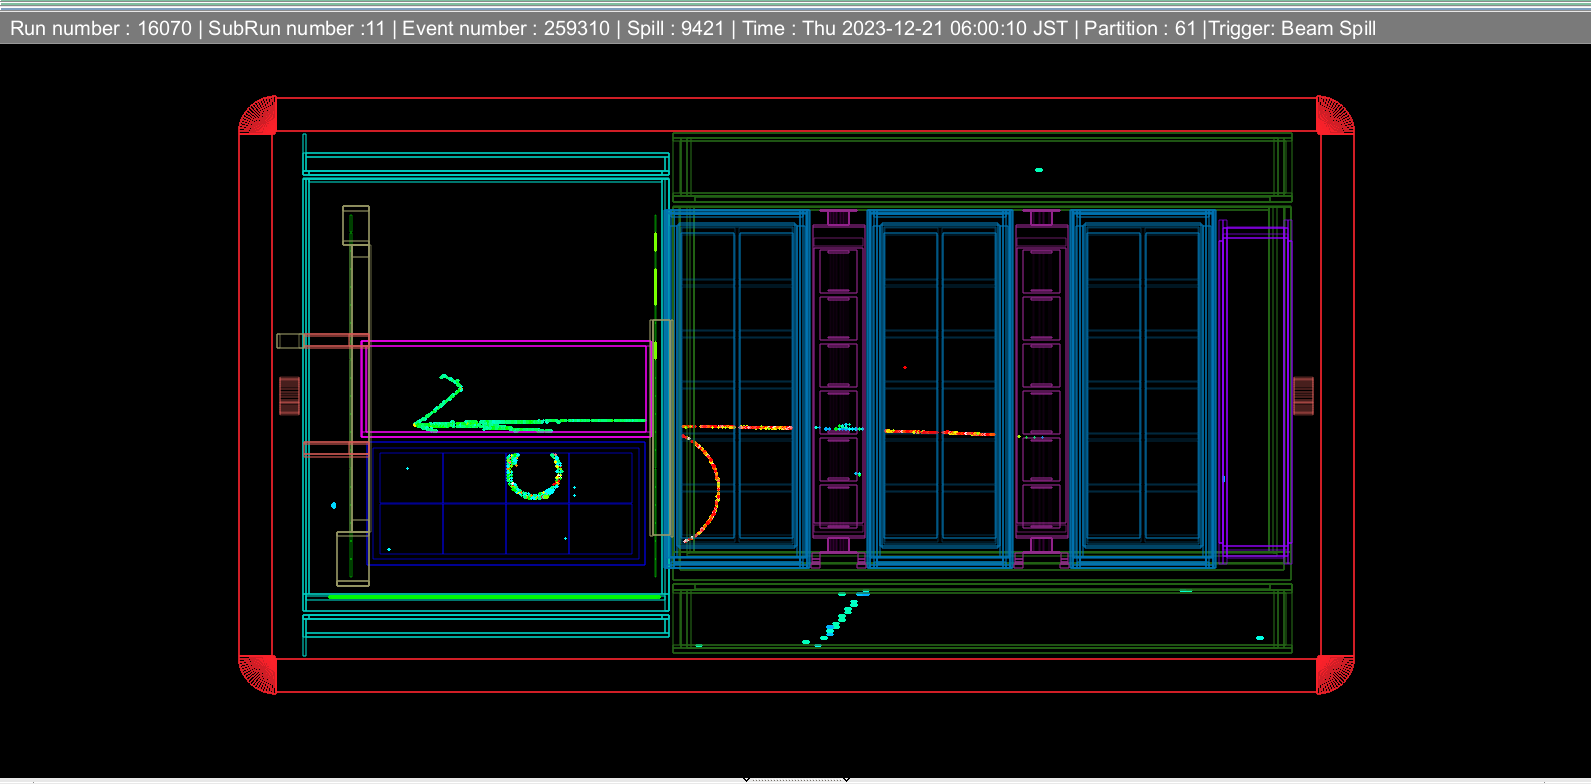
\includegraphics[width=0.5\linewidth]{fig/upgradeEvtDis.png}
        \caption{Event display of a possible $\pi^+$ event.}
        \label{fig:ndup-evedis}
    \end{figure}